\documentclass[12pt]{article}
\usepackage{scrextend}
\usepackage[utf8]{inputenc}
\usepackage[polish]{babel}
\usepackage[T1]{fontenc}%polskie znaki
\usepackage[utf8]{inputenc}%polskie znaki
\usepackage{geometry}
\usepackage{float}
\usepackage{enumitem}
\usepackage{hyperref}
\usepackage{graphicx}
\usepackage{tabulary}
\usepackage{etoc}
\usepackage[normalem]{ulem} 
\usepackage{tikz}
\usepackage[bf]{caption}
\usepackage{listings}
\renewcommand{\baselinestretch}{1.5}
\usepackage{amsmath}% http://ctan.org/pkg/amsmath
\usepackage{array}% http://ctan.org/pkg/array
\usepackage{listings}
\usepackage{xcolor}
 
\definecolor{codegreen}{rgb}{0,0.6,0}
\definecolor{codegray}{rgb}{0.5,0.5,0.5}
\definecolor{codepurple}{rgb}{0.58,0,0.82}
\definecolor{backcolour}{rgb}{0.95,0.95,0.92}
 
\lstdefinestyle{mystyle}{
    backgroundcolor=\color{backcolour},   
    commentstyle=\color{codegreen},
    keywordstyle=\color{magenta},
    numberstyle=\tiny\color{codegray},
    stringstyle=\color{codepurple},
    basicstyle=\ttfamily\footnotesize,
    breakatwhitespace=false,         
    breaklines=true,                 
    captionpos=b,                    
    keepspaces=true,                 
    numbers=left,                    
    numbersep=5pt,                  
    showspaces=false,                
    showstringspaces=false,
    showtabs=false,                  
    tabsize=2,
    postbreak=\mbox{\textcolor{red}{$\hookrightarrow$}\space}
}
\renewcommand{\lstlistlistingname}{Spis listingów}\lstset{style=mystyle}

\graphicspath{ {img/} }
\newgeometry{lmargin=2.0cm, rmargin=2.0cm, tmargin=2.0cm, bmargin=2.0cm}
\clubpenalty=9996
\widowpenalty=9999
\brokenpenalty=4991
\predisplaypenalty=10000
\postdisplaypenalty=1549
\displaywidowpenalty=1602

\title{ 
    \vspace*{55mm}
    \textsc{
        \textbf{Urządzenia Peryferyjne}\\
        \large Sprawozdanie  \\
        \Large RaspberryPi
        }
} 
\author{
Damian Koper,  241292\\
Wiktor Pieklik, 241282\\
}

\date{\today}

\begin{document}
\maketitle

\newpage
\localtableofcontents
\listoffigures
\lstlistoflistings

\newpage

\section{Cel ćwiczenia}
Celem ćwiczenia było zapoznanie się z urządzeniem RaspberryPi w wersji 4B\cite{raspi}. Należało obsłużyć miganie diodą z poziomu powłoki systemowej, języka Python oraz wykonać pomiar temperatury i odległości z wykorzystaniem odpowiednich sensorów.

\section{RaspberryPi}
RaspberryPi to komputer umieszczony na płytce o wymiarach 85,60 x 56,50 mm. Posiada on 64-bitowy czterordzeniowy procesor Cortex-A72 wykorzystujący architekturę ARM\cite{arm}. W zależności od wersji posiada od 1GB do 4GB pamięci RAM. RaspberryPi wyposażone jest również w port Ethernet, 3.5mm jack oraz 2x micro HDMI, interfejs CSI oraz DSI. Posiada również wyprowadzenia na 40 pinów, które realizują wiele popularnych interfejsów oraz mogą być wykorzystywane w dowolny sposób.

\begin{figure}[h]
  \centering
  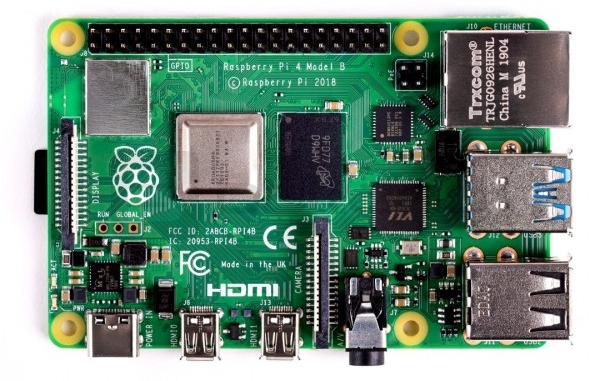
\includegraphics[width=0.5\linewidth]{raspi}
  \caption{RaspberryPi w wersji 4B\cite{raspi:img}.}
  \label{raspi:1}
\end{figure}
\clearpage
\subsection{Piny}
W RaspberryPi wyprowadzone piny odpowiedzialne są za:
\begin{itemize}[noitemsep]
  \item wyprowadzenie masy,
  \item zasilanie 3.3V i 5V,
  \item interfejs UART,
  \item interfejs I$^2$C,
  \item interfejs SPI.
\end{itemize}
Rysunek \ref{raspi:2} prezentuje jak rozmieszczone są piny odpowiedzialne za poszczególne funkcje. Piny GPIO (General Purpose IO) mogą być używane jako piny wejściowe lub wyjściowe, mogą również pełnić funkcje zegara lub stać się wyjściem działającym w trybie PWM.

\begin{figure}[h]
  \centering
  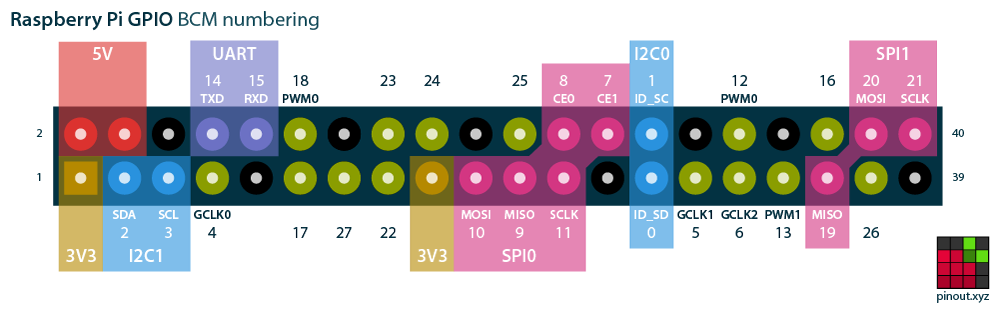
\includegraphics[width=\linewidth]{raspberry-pi-pinout}
  \caption{Piny RaspberryPi w wersji 4B\cite{pinout}.}
  \label{raspi:2}
\end{figure}

\subsection{System operacyjny}
Na RaspberryPi uruchomione mogą zostać systemy skompilowane na architekturę ARM. Najpopularniejsze z nich oparte są na Linuxie, jednym z nich jest system Raspbian\cite{raspbian}. Na RaspberryPi może uruchomiony również zostać system Windows 10 w wersji \textit{Internet of Things}\cite{w10iot}.
\newpage
\section{Dioda LED}
Podstawowa obsługa diody LED polegała na włączaniu i wyłączaniu jej co sekundę. Układ został podłączony zgodnie ze schematem z rysunku \ref{sch:1}. Do zaświecenia diodą wystarczy prąd płynący przy ustawieniu stanu pinu GPIO na wysoki. Pin GPIO na wyjściu dostarcza napięcie 3.3V i może obsłużyć natężenie maksymalnie 50mA\cite{raspi:power}.

\begin{figure}[h]
  \centering
  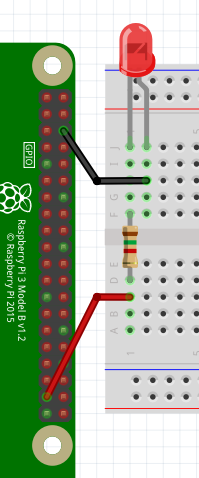
\includegraphics[height=0.4\linewidth]{sch1}
  \caption{Podłączenie diody LED.}
  \label{sch:1}
\end{figure}

\subsection{Sterowanie z poziomu powłoki systemowej}
Jądro Linuxa domyślnie wyposażone jest w sterowniki obsługujące interface GPIO. Jego cechą, tak jak wszystkich systemach operacyjnych opartych na Unixie, jest obsługa urządzeń poprzez interface udostępniany użytkownikowi w postaci pliku. Sprowadza to obsługę urządzenia do wykonywania operacji odczytu i zapisu do określonych plików.

W przypadku obsługi diody LED w pierwszej kolejności należało aktywować odpowiedni pin w trybie wyjścia (linie 3 i 4 na listingu \ref{lst:bash}). Następnie w nieskończonej pętli skrypt zapisywał do pliku przypisanego do aktywowanego pinu wartości \lstinline{0} i \lstinline{1}. Skutkowało to zmianą napięcia na wyjściu, a w konsekwencji zapalenie i gaśnięcie diody.
%\newpage
\lstinputlisting[language=Bash, caption={Obsługa diody LED z poziomu powłoki systemowej.}, label=lst:bash]{code/led.sh}

\subsection{Sterowanie z poziomu języka Python}
Sterowanie diodą z poziomu języka Python odbywa się na podobnej zasadzie co wcześniej. Użyta biblioteka RPi.GPIO posiada API, które wewnętrznie również korzysta ze sterowników jądra systemu operacyjnego. 
\lstinputlisting[language=Python, caption={Obsługa diody LED z poziomu jezyka Python.}, label=lst:python]{code/led.py}

Wywołanie funkcji \lstinline{GPIO.setmode} odpowiada za ustawienie mapowania numeru pinu na jego fizyczny odpowiednik. Funkcja \lstinline{GPIO.setup} ustawia kierunek i początkową wartość dla pinu, a funkcja \lstinline{GPIO.output} zmienia wyjście pinu na wartość z argumentu.
\newpage
\subsection{Sterowanie przyciskiem}

Sterowanie diodą za pomocą przycisku wymagało dodania do układu przycisku wraz z rezystorem, który ogranicza przepływ prądu. Jeden koniec podłączono pod pin zasilający 3.3V, a drugi do pinu GPIO, za pomocą którego odczytywany był stan naciśnięcia przycisku. Schemat podłączenia pokazany został na rysunku \ref{sch:2}.

\begin{figure}[h]
  \centering
  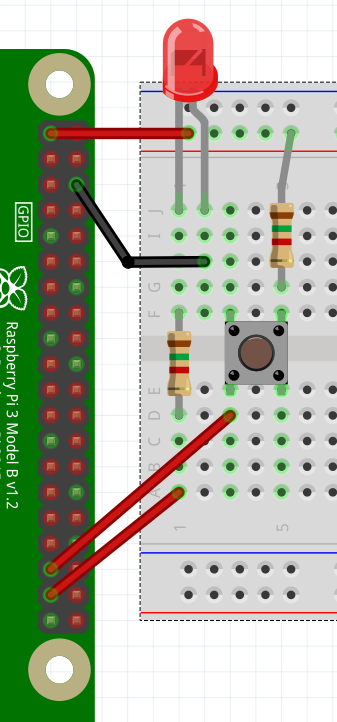
\includegraphics[height=0.4\linewidth]{sch2}
  \caption{Podłączenie diody LED i przycisku.}
  \label{sch:2}
\end{figure}

Zdarzenie naciśnięcia przycisku obsługiwane było za pomocą przerwania. Było ono wywoływane przy rosnącym zboczu sygnału. Za konfigurację tego zachowania odpowiada metoda \lstinline{GPIO.add_event_detect} wywołana w linii 17 listingu \ref{lst:button}, która w trzecim argumencie przyjmuje funkcję obsługi zdarzenia. Stan diody przechowywany był w zmiennej typu \lstinline{boolean} i zmieniany był na przeciwny przy każdym naciśnięciu przycisku.

\lstinputlisting[language=Python, caption={Sterowanie diodą LED za pomocą przycisku. Najważniejsze fragmenty.}, label=lst:button, linerange={8-24}]{code/led_button.py}

Naciśnięcie przycisku nie powoduje od razu idealnego zwarcia. Występują wtedy zakłócenia powstawania zbocza rosnącego, które mogą powodować wielokrotne wykrycie zdarzenia tego samego naciśnięcia przycisku. W celu wyeliminowania tego zjawiska w linii 6 listingu \ref{lst:button} następuje oczekiwania na ustabilizowanie się sygnału przed jego odczytem wynoszące 15 milisekund.

\section{Pomiar temperatury}
Pomiar temperatury odbywał się z wykorzystaniem termometru DS18B20\cite{term} komunikującego się z RaspberryPi poprzez protokół 1-Wire. Jest to protokół pozwalający na komunikację tylko z wykorzystaniem, oprócz złącza masy, jednego przewodu wykorzystując zasilanie pasożytnicze. W wypadku podłączonego układu napięcie zasilające dostarczane jest osobnym złączem $V_{dd}$.
\begin{figure}[h]
  \centering
  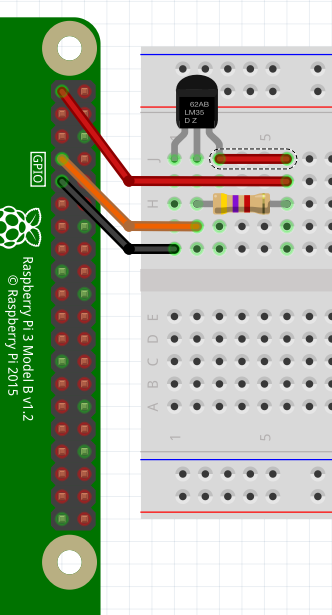
\includegraphics[height=0.4\linewidth]{sch3}
  \caption{Podłączenie termometru.}
  \label{sch:3}
\end{figure}

Obsługę protokołu 1-Wire należy włączyć w opcjach konfiguracyjnych systemu Raspbian, a przewód transmisji danych musi być podłączony do pinu GPIO nr 4. Każde urządzenie identyfikowane jest 64-bitowym numerem, dzięki czemu istnieje możliwość podłączenia pod jedną magistralę wielu urządzeń. Aby odczytać temperaturę należy wyświetlić zawartość pliku \lstinline{/sys/bus/w1/devices/XXX/w1_slave}, gdzie \lstinline{XXX} to numer urządzenia. Plik ten jest automatycznie aktualizowany przez system.

Aby odczytać temperaturę w języku Python wykorzystano bibliotekę \lstinline{w1thermsensor}, która pozwala stworzyć obiekt typu \lstinline{W1ThermSensor}, który metodą \lstinline{get_temperature} pozwala odczytać temperaturę w stopniach Celsjusza. Odczyt przeprowadzany jest co sekundę. Cały kod za to odpowiedzialny widoczny jest na listingu \ref{lst:term}.
\lstinputlisting[language=Python, caption={Odczytywanie temperatury.}, label=lst:term]{code/w1_therm.py}

\section{Pomiar odległości i dioda RGB}

Na rysunku \ref{sch:4} pokazano połączenie sensora HC-SR04\cite{ultrasonic}. Zasilany jest on napięciem 5V i oprócz pinów $V_{CC}$ i GND ma on jeszcze wyprowadzenia Trigger i Echo. Pierwsze z nich odpowiada za rozpoczęcie pomiaru, a drugie informuje o jego zakończeniu. Pomiar zakończony jest wtedy, kiedy wysłana i odbita od obiektu fala dźwiękowa wyemitowana przez sensor do niego wróci. Znając prędkość dźwięku w powietrzu i moment rozpoczęcia pomiaru możemy na tej podstawie wyliczyć odległość.


\begin{figure}[H]
  \centering
  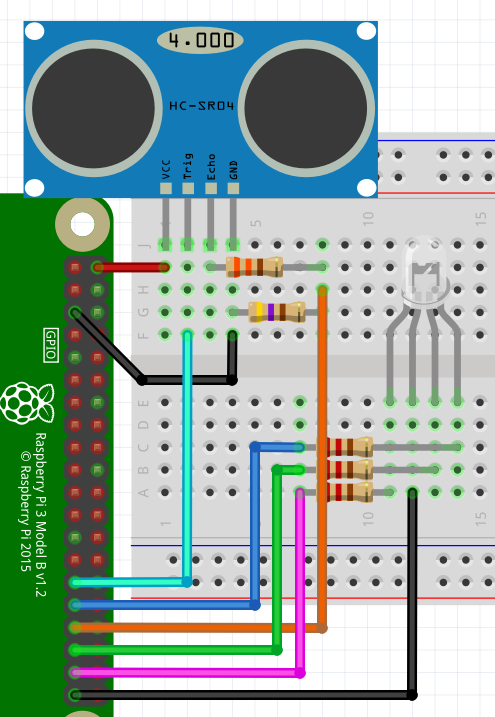
\includegraphics[height=0.4\linewidth]{sch4}
  \caption{Podłączenie sensora HC-SR04 i diody RGB.}
  \label{sch:4}
\end{figure}

Na rysunku \ref{sch:4} widać również podłączenie diody RGB LED, gdzie każdym kolorem steruje osobny pin GPIO.

\begin{lstlisting}[language=Python, caption={Odczytywanie odległości.}, label=lst:ultrasonic]
def distance():
    GPIO.output(GPIO_TRIGGER, True)
    time.sleep(0.00001)
    GPIO.output(GPIO_TRIGGER, False)
 
    StartTime = time.time()
    StopTime = time.time()
    while GPIO.input(GPIO_ECHO) == 0:
        StartTime = time.time()
    while GPIO.input(GPIO_ECHO) == 1:
        StopTime = time.time()
 
    TimeElapsed = StopTime - StartTime
    distance = (TimeElapsed * 34300) / 2
    return distance
\end{lstlisting}
\clearpage
Pokazana na listingu \ref{lst:ultrasonic} metoda \lstinline{distance} włącza pomiar wysyłając impuls o długości $10\mu s$. Następnie czeka na stan wysoki na pinie Echo, który informuje o dotarciu odbitej fali. Na podstawie czasów tych wydarzeń obliczana jest odległość wg wzoru \ref{eq:1}.
\begin{gather}
  \label{eq:1}
d = ((t_k - t_s) \cdot 34300)/2
\intertext{Gdzie:}
  \begin{tabular}{>{$}r<{$}@{\ :\ }l}
    d & szukana odległość \\
    t_{k} & czas końca pomiaru \\
    t_{s} & czas początku pomiaru \\
    34300[\frac{cm}{s}] & prędkość dźwięku w powietrzu wyrażona w centymetrach na sekundę \\
  \end{tabular}\nonumber
\end{gather}

Wynik dzielony jest na dwa, ponieważ otrzymany czas zawiera drogę fali do obiektu i od niego po odbiciu.

Na podstawie odczytanej odległości odbywało się sterowanie kolorem świecenia diody RGB. Co sekundę wykonywany był pomiar i w zależności od odległości dioda świeciła na czerwono lub zielono. Kod odpowiedzialny za to zachowanie znajduje się w listingu \ref{lst:ultrasonicRGB}.
\begin{lstlisting}[language=Python, caption={Odczytywanie odległości - sterowanie diodą.}, label=lst:ultrasonicRGB]
while True: 
    dist = distance()
    if dist < 20:
        GPIO.output(rpin, GPIO.HIGH)
        GPIO.output(gpin, GPIO.LOW)
    else:
        GPIO.output(rpin, GPIO.LOW)
        GPIO.output(gpin, GPIO.HIGH)
    print ("Measured Distance = %.1f cm" % dist)
    time.sleep(1)
\end{lstlisting}

\newpage
\section{Podsumowanie}
Komputer RaspberryPi ze względu na swoją cenę, mały rozmiar i rozbudowaną społeczność użytkowników stanowi doskonałe źródło edukacyjne, pozwalające poznać niskopoziomowe mechanizmy, protokoły i interfejsy. Pracując z w pełni funkcjonalnym systemem operacyjnym RaspberryPi nie ogranicza możliwości użycia jej również w wysokopoziomowych projektach. 

Model RaspberryPi w wersji 4B ma jednak wadę, którą jest nieodpowiedni odpływ ciepła z procesora. Skutkowało to przegrzewaniem się układu, który w celu ochłodzenia obniżał swoje taktowanie. Działo się to przy bardziej wymagających obliczeniowo zadaniach, którymi okazały się otwarcie kilku stron internetowych.

\newpage
\begin{thebibliography}{9}
  \bibitem{raspi}
  RaspberryPi: \url{https://pl.wikipedia.org/wiki/Raspberry_Pi}
  \bibitem{arm}
  ARM: \url{https://pl.wikipedia.org/wiki/Architektura_ARM}
  \bibitem{raspi:img}
  RaspberryPi - wygląd: \url{https://botland.com.pl/59269-thickbox_default/raspberry-pi-4-model-b-wifi-dualband-bluetooth-4gb-ram-15ghz.jpg}
  \bibitem{pinout}
  Pinout: \url{http://pinout.xyz}
  \bibitem{raspbian}
  Raspbian: https://www.raspbian.org/
  \bibitem{w10iot}
  Windows 10 IoT: \url{https://docs.microsoft.com/pl-pl/windows/iot-core/}
  \bibitem{raspi:power}
  Power pins: \url{https://elinux.org/RPi_Low-level_peripherals#Power_pins}
\end{thebibliography}
\end{document}